%% Rebuild the result figures without the manuscript.
%%   pdflatex standalone.tex
%% Produces one page per figure, using the coordinates in
%% ../sim/results/pgfplots.tex — i.e. whatever the last experiment run wrote.
\documentclass[journal]{IEEEtran}
\usepackage{amsmath,amssymb,graphicx,tikz}
\usepackage{pgfplots}\pgfplotsset{compat=1.18}
\newcommand{\SP}{\textsc{Slice-Purify}}
\newcommand{\DMC}{\textsc{DMC}}
%% math macros the figure files borrow from the manuscript preamble
\newcommand{\R}{\mathbb{R}}
\newcommand{\E}{\mathbb{E}}
\newcommand{\Prb}{\mathbb{P}}
\newcommand{\Ind}{\mathbb{1}}
\pgfplotsset{
    sp/.style={color=blue,           mark=o,        thick, mark size=1.6},
    b1/.style={color=red,            mark=square,   thick, mark size=1.6, dashed},
    b2/.style={color=green!60!black, mark=triangle, thick, mark size=1.8, dash dot},
    b3/.style={color=orange,         mark=diamond,  thick, mark size=1.8, densely dotted},
    ref/.style={color=gray, thin, dashed, mark=none},
    axstd/.style={
        width=\columnwidth, height=5.4cm,
        grid=major, grid style={dotted,gray!40},
        legend style={font=\scriptsize, fill opacity=0.85,
                      text opacity=1, draw=gray!50},
        tick label style={font=\footnotesize},
        label style={font=\small}}}
%% Auto-generated by sim/experiments.py - do not edit by hand.
\def\Eoneasrnone{(2,0.1875) (6,0.28) (10,0.4) (14,0.4194) (18,0.4603) (22,0.4921)}
\def\Eoneasrpur{(2,0.0625) (6,0.08) (10,0.05) (14,0.0161) (18,0.0) (22,0.0)}
\def\Eoneasrfull{(2,0.0) (6,0.0) (10,0.0) (14,0.0) (18,0.0) (22,0.0)}
\def\Eonepsnrbenign{(2,11.4761) (6,13.1135) (10,16.0522) (14,19.1948) (18,22.7119) (22,25.3424)}
\def\Eonepsnrpur{(2,10.8105) (6,11.6151) (10,13.7564) (14,15.4504) (18,16.5434) (22,17.1464)}
\def\Eoneaccnone{(2,0.125) (6,0.2) (10,0.2) (14,0.2581) (18,0.1587) (22,0.1905)}
\def\Eoneaccfull{(2,0.75) (6,0.88) (10,0.95) (14,0.9839) (18,1.0) (22,1.0)}
\def\Etwoasrnodef{(0.0,0.8571) (0.2,0.7143) (0.4,0.5079) (0.6,0.3387) (0.8,0.4762) (1.0,0.7937)}
\def\Etwoasrpur{(0.0,0.0) (0.2,0.0) (0.4,0.0) (0.6,0.0) (0.8,0.1746) (1.0,0.7937)}
\def\Etwodone{(0.0,222.7714) (0.2,116.7207) (0.4,53.8847) (0.6,18.7923) (0.8,3.7847) (1.0,0.473)}
\def\Etwodtwo{(0.0,0.7452) (0.2,5.5147) (0.4,14.5517) (0.6,23.9706) (0.8,28.9077) (1.0,27.0436)}
\def\Etwofused{(0.0,2.8819) (0.2,3.1827) (0.4,3.2648) (0.6,3.006) (0.8,2.4187) (1.0,1.8322)}
\def\Etwodpsnr{(0.0,-0.0288) (0.2,1.0641) (0.4,2.0129) (0.6,3.2257) (0.8,4.6356) (1.0,6.0778)}
\def\Ethreeasr{(0,0.3968) (1,0.0635) (2,0.0323) (3,0.0476) (4,0.0323) (6,0.0476) (8,0.0323) (12,0.0159)}
\def\Ethreepsnr{(0,14.7161) (1,15.3089) (2,15.3943) (3,15.4362) (4,15.3719) (6,15.4965) (8,15.4674) (12,15.513)}
\def\Ethreessim{(0,0.3517) (1,0.3705) (2,0.3768) (3,0.3763) (4,0.3735) (6,0.3771) (8,0.3789) (12,0.379)}
\def\Ethreems{(0,1.2104) (1,3.1459) (2,4.7626) (3,6.4461) (4,8.0562) (6,11.5045) (8,16.0344) (12,22.6907)}
\def\Ethreesep{(0,1.0) (1,4.5323) (2,9.0709) (3,8.5576) (4,8.1861) (6,6.5284) (8,5.5316) (12,5.1668)}
\def\Ethreepsnrbenign{(0,19.3856) (1,19.2231) (2,19.3725) (3,19.6084) (4,19.1615) (6,19.5047) (8,19.5569) (12,19.37)}
\def\Efourdone{(0.0,0.0) (0.006,0.6383) (0.012,0.645) (0.018,0.655) (0.024,0.6617) (0.028,0.6617) (0.034,0.6767) (0.04,0.6833) (0.046,0.6867) (0.05,0.69) (0.114,0.7817) (0.178,0.7983) (0.24,0.805) (0.304,0.805) (0.368,0.8067) (0.43,0.8083) (0.494,0.8183) (0.558,0.8217) (0.62,0.835) (0.684,0.85) (0.748,0.8583) (0.81,0.8917) (0.874,0.9383) (0.938,0.9817) (1.0,1.0)}
\def\Efourdtwo{(0.0,0.0) (0.006,0.7917) (0.012,0.7917) (0.018,0.7933) (0.024,0.7967) (0.028,0.7967) (0.034,0.7967) (0.04,0.7983) (0.046,0.8) (0.05,0.8) (0.114,0.81) (0.178,0.82) (0.24,0.8367) (0.304,0.85) (0.368,0.8667) (0.43,0.8867) (0.494,0.8967) (0.558,0.91) (0.62,0.925) (0.684,0.945) (0.748,0.9567) (0.81,0.9617) (0.874,0.9733) (0.938,0.9867) (1.0,1.0)}
\def\Efourfused{(0.0,0.0) (0.006,0.995) (0.012,0.995) (0.018,0.9967) (0.024,0.9967) (0.028,0.9967) (0.034,0.9967) (0.04,0.9967) (0.046,0.9967) (0.05,0.9967) (0.114,0.9983) (0.178,0.9983) (0.24,0.9983) (0.304,0.9983) (0.368,0.9983) (0.43,0.9983) (0.494,0.9983) (0.558,0.9983) (0.62,1.0) (0.684,1.0) (0.748,1.0) (0.81,1.0) (0.874,1.0) (0.938,1.0) (1.0,1.0)}
\def\Efivepoisoned{(1,0.6) (2,0.5) (3,0.4286) (4,0.375) (5,0.3333) (6,0.3) (7,0.2727) (8,0.25) (9,0.2308) (10,0.2143) (11,0.2) (12,0.1875) (13,0.1765) (14,0.1667) (15,0.1579) (16,0.15) (17,0.1429) (18,0.1364) (19,0.1304) (20,0.125) (21,0.12) (22,0.1154) (23,0.1111) (24,0.1071) (25,0.1034) (26,0.1) (27,0.0968) (28,0.0938) (29,0.0909) (30,0.0882) (31,0.0857) (32,0.0833) (33,0.0811) (34,0.0789) (35,0.0769) (36,0.075) (37,0.0732) (38,0.0714) (39,0.0698) (40,0.0682)}
\def\Efivebenign{(1,0.6) (2,0.6667) (3,0.7143) (4,0.75) (5,0.7778) (6,0.8) (7,0.8182) (8,0.8333) (9,0.8462) (10,0.8571) (11,0.8667) (12,0.875) (13,0.8824) (14,0.8889) (15,0.8947) (16,0.9) (17,0.9048) (18,0.9091) (19,0.913) (20,0.9167) (21,0.92) (22,0.9231) (23,0.9259) (24,0.9286) (25,0.931) (26,0.9333) (27,0.9355) (28,0.9375) (29,0.9394) (30,0.9412) (31,0.9429) (32,0.9444) (33,0.9459) (34,0.9474) (35,0.9487) (36,0.95) (37,0.9512) (38,0.9524) (39,0.9535) (40,0.9545)}
\def\Efivedagentic{(1,15.29) (2,6.43) (4,6.29) (8,3.29) (16,2.07)}
\def\Efivedrandom{(1,14.21) (2,11.64) (4,6.14) (8,4.0) (16,3.07)}
\def\Efivedpassive{(1,13.14) (2,9.5) (4,5.79) (8,3.79) (16,2.29)}
\def\Esixundef{(10,0.0) (20,0.0) (30,0.0) (40,0.0) (50,0.0) (60,0.0) (70,5e-05) (80,0.01479) (90,0.46383)}
\def\Esixstatic{(10,0.00555) (20,0.0156) (30,0.03205) (40,0.06875) (50,0.1089) (60,0.18455) (70,0.28605) (80,0.463) (90,0.6877)}
\def\Esixfull{(10,0.0) (20,0.0) (30,0.0) (40,0.00055) (50,0.0024) (60,0.00635) (70,0.02435) (80,0.1085) (90,0.3322)}
\def\Esevenfused{(10,0.111) (25,0.109) (50,0.14) (100,0.241) (200,0.386) (400,0.866) (800,1.297)}
\def\Esevenpertenant{(10,0.339) (25,0.841) (50,1.79) (100,3.436) (200,8.913) (400,15.452) (800,29.184)}
\def\Esevenexhaustive{(10,0.6) (25,1.603) (50,3.066) (100,6.075) (200,15.259) (400,25.931) (800,50.614)}
\def\Enineasr{(0.05,0.52381) (0.1,0.53226) (0.2,0.59677) (0.35,0.52381) (0.55,0.57143)}
\def\Eninefused{(0.05,3.30394) (0.1,3.33303) (0.2,3.32669) (0.35,3.33678) (0.55,3.31229)}
\def\Enineexposure{(0.05,0.04287) (0.1,0.08563) (0.2,0.17041) (0.35,0.29416) (0.55,0.4486)}

%% cross-references the manuscript owns; stubbed so this compiles alone
\newcommand{\stubref}[1]{\textbf{?}}
\let\eqref\stubref \let\ref\stubref
\begin{document}
\begin{figure}[!t]
\centering
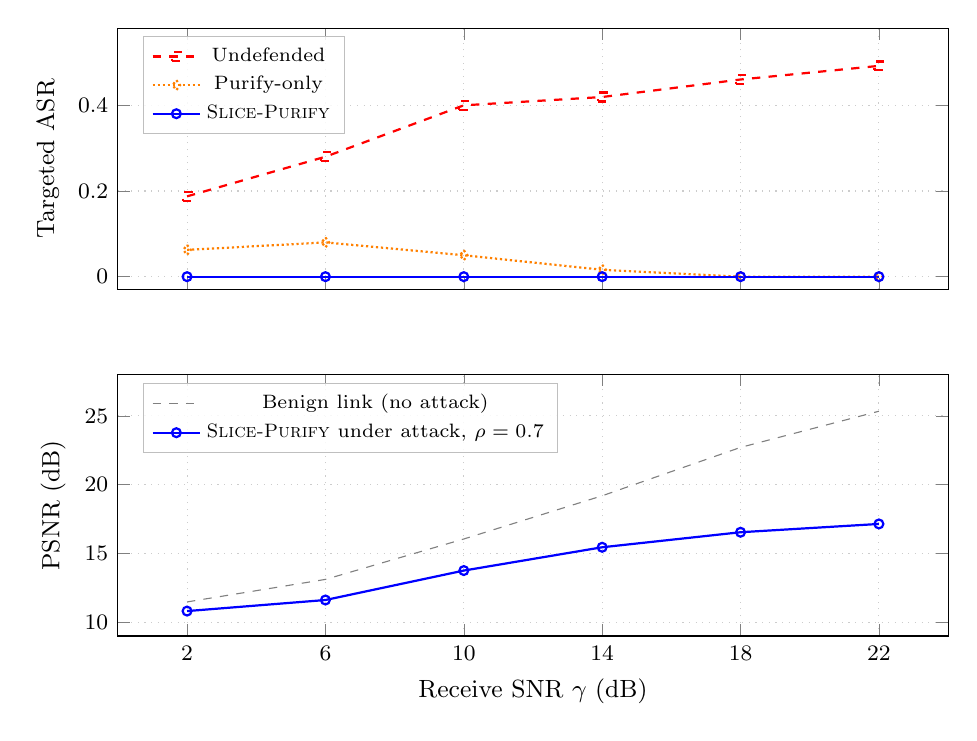
\begin{tikzpicture}
\begin{axis}[axstd, height=4.9cm,
    xlabel={}, xticklabels={},
    ylabel={Targeted ASR},
    xmin=0, xmax=24, ymin=-0.03, ymax=0.58,
    xtick={2,6,10,14,18,22},
    legend pos=north west, legend columns=1]
\addplot[b1] coordinates {\Eoneasrnone}; \addlegendentry{Undefended}
\addplot[b3] coordinates {\Eoneasrpur};  \addlegendentry{Purify-only}
\addplot[sp] coordinates {\Eoneasrfull}; \addlegendentry{\SP{}}
\end{axis}
\begin{axis}[axstd, height=4.9cm, at={(0cm,-4.4cm)},
    xlabel={Receive SNR $\gamma$ (dB)},
    ylabel={PSNR (dB)},
    xmin=0, xmax=24, ymin=9, ymax=28,
    xtick={2,6,10,14,18,22},
    legend pos=north west, legend columns=1]
\addplot[ref, mark=none] coordinates {\Eonepsnrbenign};
    \addlegendentry{Benign link (no attack)}
\addplot[sp] coordinates {\Eonepsnrpur};
    \addlegendentry{\SP{} under attack, $\rho=0.7$}
\end{axis}
\end{tikzpicture}
\caption{Attack efficacy and fidelity versus channel SNR at the
adaptive operating point $\rho=0.7$. Upper: targeted attack success
rate. Lower: reconstruction PSNR. Undefended ASR \emph{increases} with
SNR, because a good channel delivers the attacker's semantic anchor as
faithfully as it delivers the source.}
\label{fig:e1}
\end{figure}
\begin{figure}[!t]
\centering
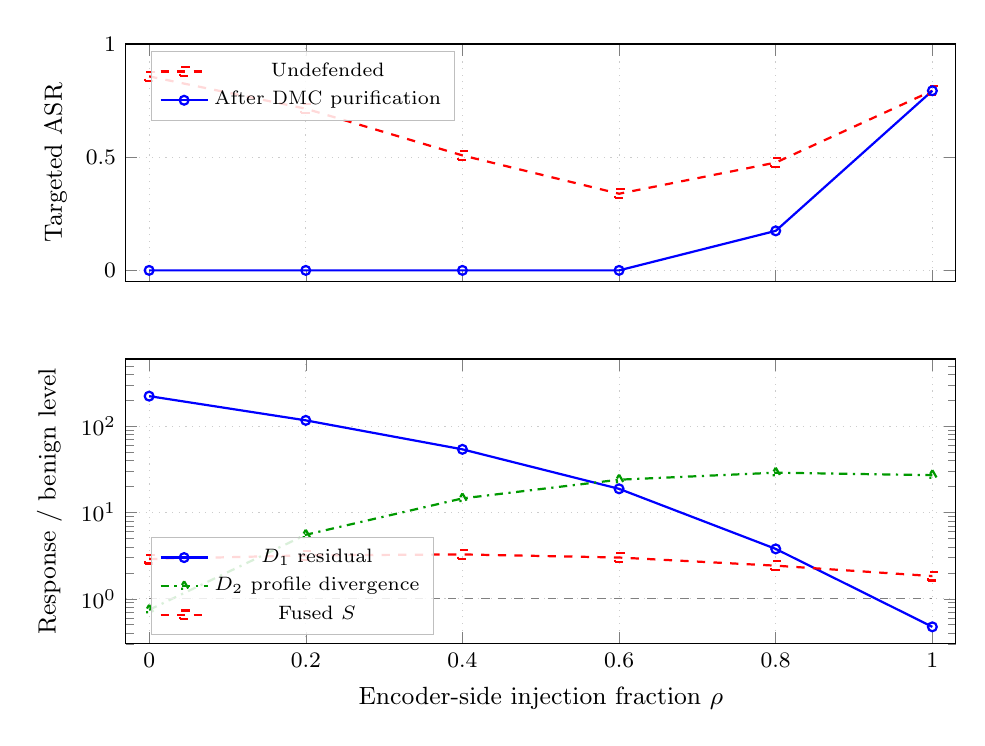
\begin{tikzpicture}
\begin{axis}[axstd, height=4.6cm,
    xlabel={}, xticklabels={},
    ylabel={Targeted ASR},
    xmin=-0.03, xmax=1.03, ymin=-0.05, ymax=1.0,
    xtick={0,0.2,0.4,0.6,0.8,1.0},
    legend pos=north west]
\addplot[b1] coordinates {\Etwoasrnodef}; \addlegendentry{Undefended}
\addplot[sp] coordinates {\Etwoasrpur};   \addlegendentry{After \DMC{} purification}
\end{axis}
\begin{axis}[axstd, height=5.2cm, at={(0cm,-4.6cm)},
    xlabel={Encoder-side injection fraction $\rho$},
    ylabel={Response / benign level},
    xmin=-0.03, xmax=1.03,
    ymode=log, ymin=0.3, ymax=600,
    xtick={0,0.2,0.4,0.6,0.8,1.0},
    legend pos=south west]
\addplot[sp] coordinates {\Etwodone};    \addlegendentry{$D_{1}$ residual}
\addplot[b2] coordinates {\Etwodtwo};    \addlegendentry{$D_{2}$ profile divergence}
\addplot[b1] coordinates {\Etwofused}; \addlegendentry{Fused $S$}
\addplot[ref] coordinates {(0,1) (1,1)};
\end{axis}
\end{tikzpicture}
\caption{The evasion--detectability frontier. Upper: purification
neutralises the attack for $\rho\le 0.6$ and fails at $\rho=1$.
Lower: the two detector responses move in opposite directions, so the
adversary must expose itself to one of them. The grey line marks the
benign level. Predicted optimal adversary:
$\rho^{\star}\approx0.74$ by \eqref{eq:rhostar}.}
\label{fig:e2}
\end{figure}
\begin{figure}[!t]
\centering
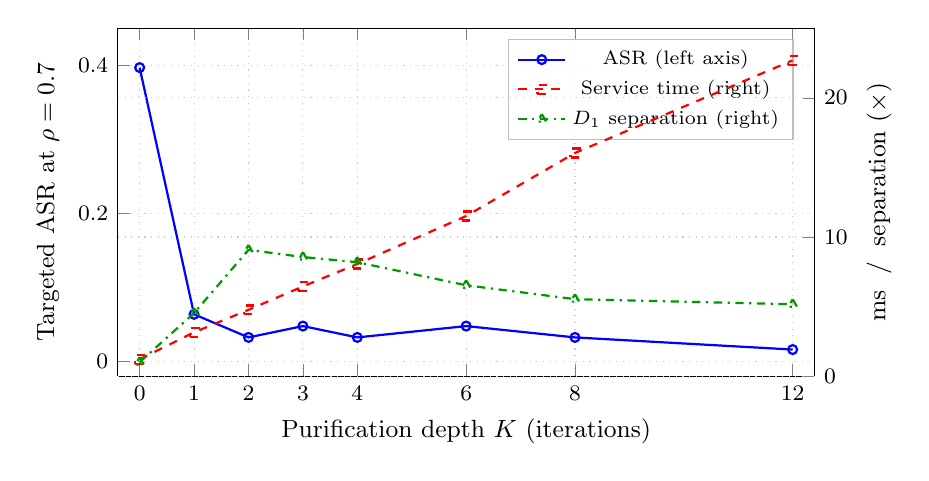
\begin{tikzpicture}
\begin{axis}[axstd, width=0.86\columnwidth, height=6.0cm,
    axis y line*=left,
    xlabel={Purification depth $K$ (iterations)},
    ylabel={Targeted ASR at $\rho=0.7$},
    xmin=-0.4, xmax=12.4, ymin=-0.02, ymax=0.45,
    xtick={0,1,2,3,4,6,8,12},
    legend pos=north east]
\addplot[sp] coordinates {\Ethreeasr};  \addlegendentry{ASR (left axis)}
\addlegendimage{b1}                     \addlegendentry{Service time (right)}
\addlegendimage{b2}                     \addlegendentry{$D_1$ separation (right)}
\end{axis}
\begin{axis}[axstd, width=0.86\columnwidth, height=6.0cm,
    axis y line*=right, axis x line=none,
    ylabel={ms \;/\; separation ($\times$)},
    xmin=-0.4, xmax=12.4, ymin=0, ymax=25]
\addplot[b1] coordinates {\Ethreems};
\addplot[b2] coordinates {\Ethreesep};
\end{axis}
\end{tikzpicture}
\caption{Purification depth trades concave security return against
linear cost. Two iterations already remove $97\%$ of the recoverable
displacement, consistent with the $(1-\eta_{c})^{K}$ decay of
\eqref{eq:kstar}; cost grows at $1.79$\,ms per iteration.}
\label{fig:e3}
\end{figure}
\begin{figure}[!t]
\centering
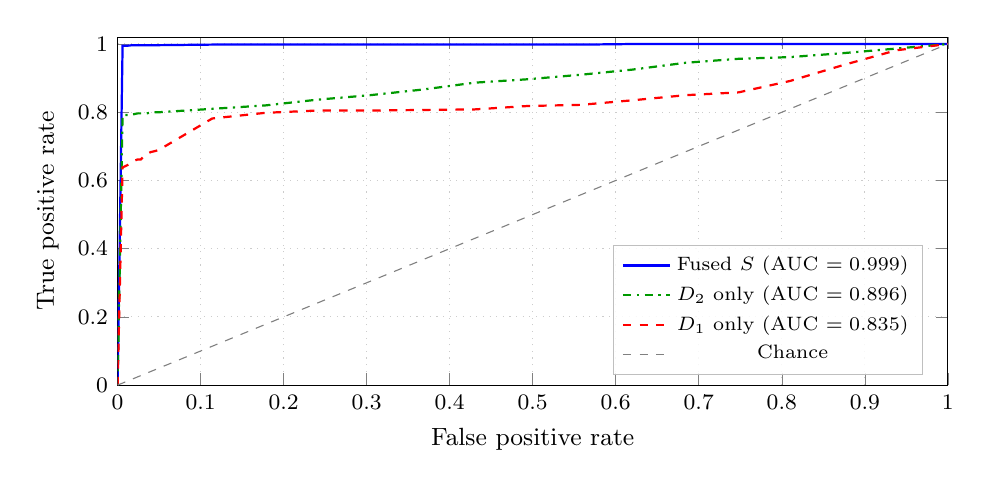
\begin{tikzpicture}
\begin{axis}[axstd, height=6.0cm,
    xlabel={False positive rate},
    ylabel={True positive rate},
    xmin=0, xmax=1, ymin=0, ymax=1.02,
    legend pos=south east]
\addplot[sp, mark=none] coordinates {\Efourfused};
    \addlegendentry{Fused $S$ (AUC $=0.999$)}
\addplot[b2, mark=none] coordinates {\Efourdtwo};
    \addlegendentry{$D_{2}$ only (AUC $=0.896$)}
\addplot[b1, mark=none] coordinates {\Efourdone};
    \addlegendentry{$D_{1}$ only (AUC $=0.835$)}
\addplot[ref] coordinates {(0,0) (1,1)};
    \addlegendentry{Chance}
\end{axis}
\end{tikzpicture}
\caption{Detector ROC over a mixture of adversary strategies
$\rho\in\{0,0.25,0.5,0.75,1\}$. Each individual statistic is blind on
half the strategy space; fusing them removes the blind spot rather
than merely averaging noise.}
\label{fig:e4}
\end{figure}

\begin{figure}[!t]
\centering
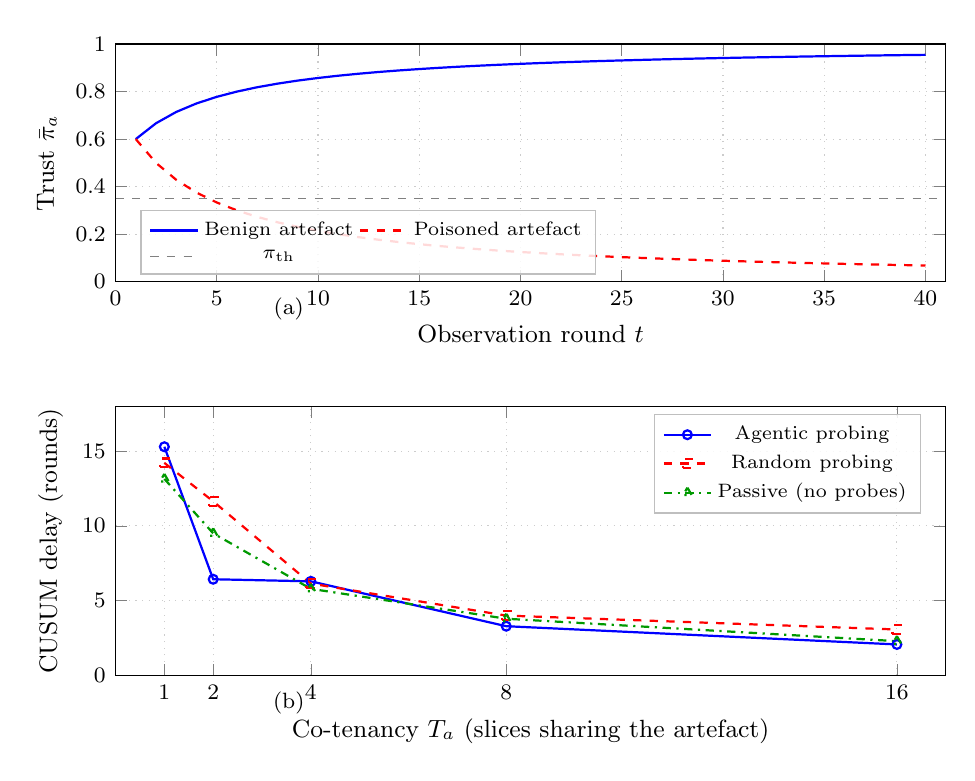
\begin{tikzpicture}
\begin{axis}[axstd, height=4.6cm,
    xlabel={Observation round $t$},
    ylabel={Trust $\bar{\pi}_{a}$},
    xmin=0, xmax=41, ymin=0, ymax=1.0,
    legend pos=south west, legend columns=2]
\addplot[sp, mark=none] coordinates {\Efivebenign};
    \addlegendentry{Benign artefact}
\addplot[b1, mark=none] coordinates {\Efivepoisoned};
    \addlegendentry{Poisoned artefact}
\addplot[ref] coordinates {(0,0.35) (41,0.35)};
    \addlegendentry{$\pi_{\mathrm{th}}$}
\end{axis}
\node[font=\footnotesize] at (2.2cm,-0.35cm) {(a)};
\begin{axis}[axstd, height=5.0cm, at={(0cm,-5.0cm)},
    xlabel={Co-tenancy $T_{a}$ (slices sharing the artefact)},
    ylabel={CUSUM delay (rounds)},
    xmin=0, xmax=17, ymin=0, ymax=18,
    xtick={1,2,4,8,16},
    legend pos=north east]
\addplot[sp] coordinates {\Efivedagentic}; \addlegendentry{Agentic probing}
\addplot[b1] coordinates {\Efivedrandom};  \addlegendentry{Random probing}
\addplot[b2] coordinates {\Efivedpassive}; \addlegendentry{Passive (no probes)}
\end{axis}
\node[font=\footnotesize] at (2.2cm,-5.35cm) {(b)};
\end{tikzpicture}
\caption{(a) Beta trust trajectories at $T_{a}=4$: separation is
established within about five rounds. (b) Detection delay against
co-tenancy at a benign average run length above $200$ rounds. Agentic
probing is the \emph{worst} policy at $T_{a}=1$, where the probe
budget displaces natural traffic before exploration pays for itself,
and the best from $T_{a}=2$ onward.}
\label{fig:e5}
\end{figure}
\begin{figure}[!t]
\centering
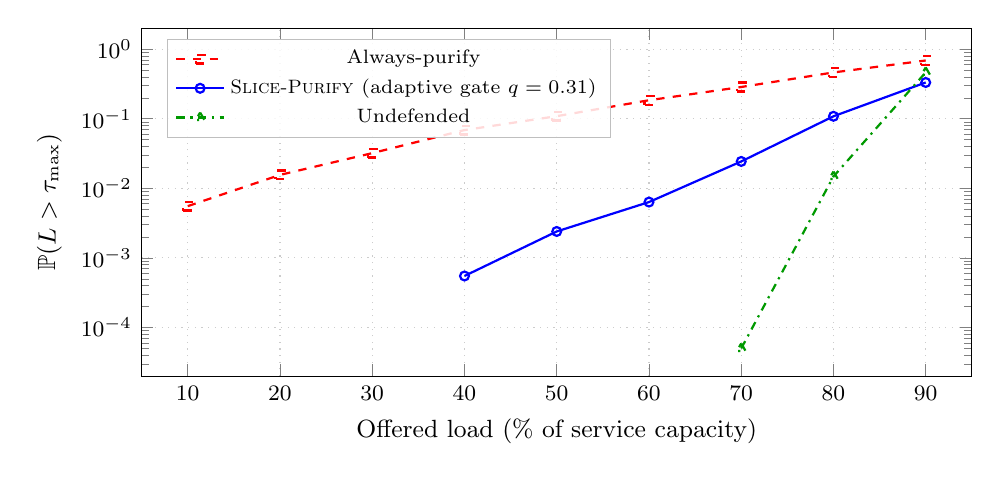
\begin{tikzpicture}
\begin{axis}[axstd, height=6.0cm,
    xlabel={Offered load (\% of service capacity)},
    ylabel={$\Prb(L > \tau_{\max})$},
    xmin=5, xmax=95,
    ymode=log, ymin=2e-5, ymax=2,
    xtick={10,20,30,40,50,60,70,80,90},
    legend pos=north west]
\addplot[b1] coordinates {\Esixstatic}; \addlegendentry{Always-purify}
\addplot[sp] coordinates {\Esixfull};   \addlegendentry{\SP{} (adaptive gate $q=0.31$)}
\addplot[b2] coordinates {\Esixundef};  \addlegendentry{Undefended}
\end{axis}
\end{tikzpicture}
\caption{Deadline-violation probability from a discrete-event
queueing simulation driven by measured service times
($1.21$\,ms decode, $8.06$\,ms purification at $K=4$,
$\tau_{\max}=25$\,ms). Below $70\%$ load the undefended arm is
strictly better---security costs tail latency. Above $80\%$ it
collapses, because corrupted frames provoke retransmissions that
compound the congestion causing them.}
\label{fig:e6}
\end{figure}
\begin{figure}[!t]
\centering
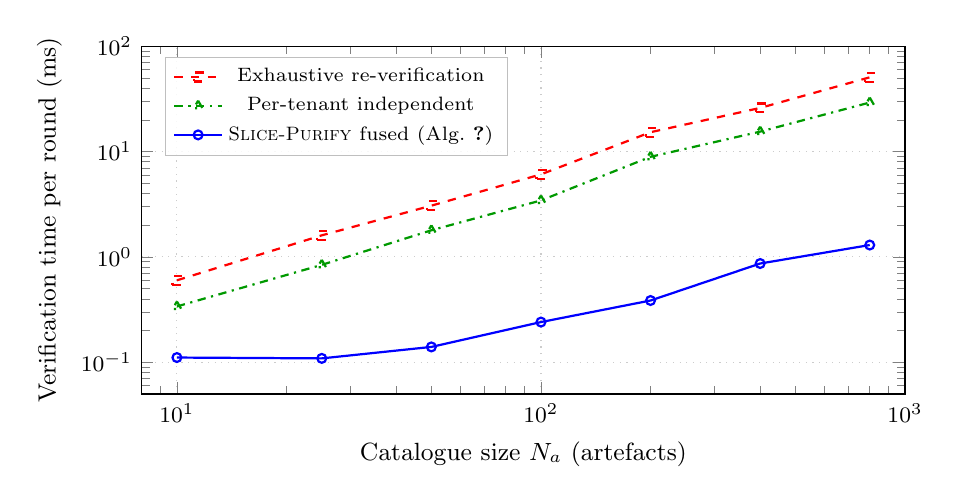
\begin{tikzpicture}
\begin{axis}[axstd, width=0.93\columnwidth, height=6.0cm,
    xlabel={Catalogue size $N_{a}$ (artefacts)},
    ylabel={Verification time per round (ms)},
    xmode=log, ymode=log,
    xmin=8, xmax=1000, ymin=0.05, ymax=100,
    legend pos=north west]
\addplot[b1] coordinates {\Esevenexhaustive};
    \addlegendentry{Exhaustive re-verification}
\addplot[b2] coordinates {\Esevenpertenant};
    \addlegendentry{Per-tenant independent}
\addplot[sp] coordinates {\Esevenfused};
    \addlegendentry{\SP{} fused (Alg.~\ref{alg:sp})}
\end{axis}
\end{tikzpicture}
\caption{Measured wall-clock cost of one orchestrator verification
round at eight co-tenants per artefact and $B=16$ gain bins. At
$N_{a}=800$ the fused scheme is $22.5\times$ faster than per-tenant
verification and $39.0\times$ faster than exhaustive re-verification,
realising the factor-$B$ saving of \eqref{eq:corch}.}
\label{fig:e7}
\end{figure}
\begin{figure}[!t]
\centering
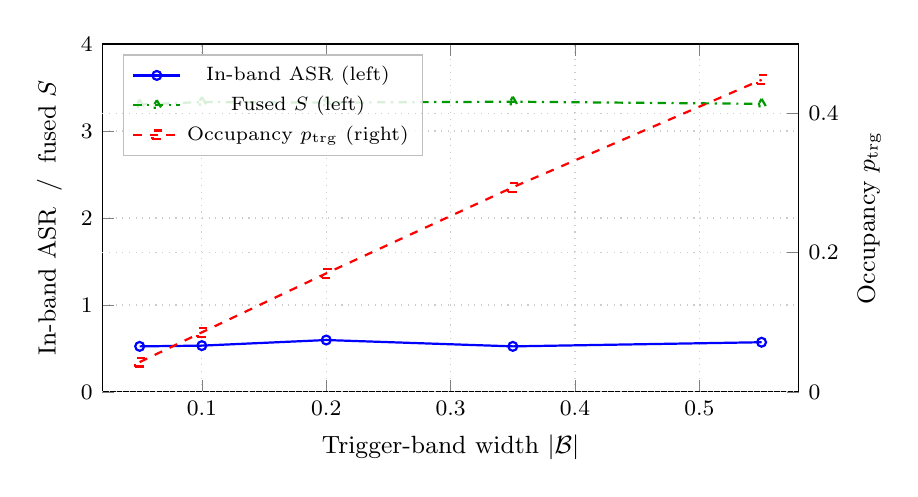
\begin{tikzpicture}
\begin{axis}[axstd, width=0.86\columnwidth, height=6.0cm,
    axis y line*=left,
    xlabel={Trigger-band width $|\mathcal{B}|$},
    ylabel={In-band ASR \;/\; fused $S$},
    xmin=0.02, xmax=0.58, ymin=0, ymax=4.0,
    legend pos=north west]
\addplot[sp] coordinates {\Enineasr};   \addlegendentry{In-band ASR (left)}
\addplot[b2] coordinates {\Eninefused}; \addlegendentry{Fused $S$ (left)}
\addlegendimage{b1}                     \addlegendentry{Occupancy $p_{\mathrm{trg}}$ (right)}
\end{axis}
\begin{axis}[axstd, width=0.86\columnwidth, height=6.0cm,
    axis y line*=right, axis x line=none,
    ylabel={Occupancy $p_{\mathrm{trg}}$},
    xmin=0.02, xmax=0.58, ymin=0, ymax=0.5]
\addplot[b1] coordinates {\Enineexposure};
\end{axis}
\end{tikzpicture}
\caption{Attacker stealth budget. Conditional on a frame falling in
the trigger band, neither attack efficacy nor detectability depends on
the band's width; what the width controls is occupancy, which scales
the attacker's reachable volume and the defender's observation rate
identically. Halving the band halves both.}
\label{fig:e9}
\end{figure}

\end{document}
